\documentclass{article}


%                                                           _..._                   
%                                                        .-'_..._''.                
%              _..._                             .--.  .' .'      '.\    .          
%            .'     '.                           |__| / .'             .'|          
%           .   .-.   .    .-''` ''-.    .-,.--. .--.. '             .'  |          
%           |  '   '  |  .'          '.  |  .-. ||  || |            <    |          
%   _    _  |  |   |  | /              ` | |  | ||  || |             |   | ____     
%  | '  / | |  |   |  |'                '| |  | ||  |. '             |   | \ .'     
% .' | .' | |  |   |  ||         .-.    || |  '- |  | \ '.          .|   |/  .      
% /  | /  | |  |   |  |.        |   |   .| |     |__|  '. `._____.-'/|    /\  \     
%|   `'.  | |  |   |  | .       '._.'  / | |             `-.______ / |   |  \  \    
%'   .'|  '/|  |   |  |  '._         .'  |_|                      `  '    \  \  \   
% `-'  `--' '--'   '--'     '-....-'`                               '------'  '---' 

\usepackage{arxiv}

\usepackage[utf8]{inputenc} % allow utf-8 input
\usepackage[T1]{fontenc}    % use 8-bit T1 fonts
\usepackage{hyperref}       % hyperlinks
\usepackage{url}            % simple URL typesettingf
\usepackage{booktabs}       % professional-quality tables
\usepackage{amsfonts}       % blackboard math symbols
\usepackage{nicefrac}       % compact symbols for 1/2, etc.
\usepackage{microtype}      % microtypography
\usepackage{lipsum}
\usepackage{graphicx}
\usepackage{tabularx}
\usepackage{wrapfig}

\usepackage[export]{adjustbox}

\usepackage{xcolor}         % http://ctan.org/pkg/xcolor

\hypersetup{
  colorlinks=true,
  linkcolor=blue!50!red,
  urlcolor=green!70!black
}

\title{lit3rick: an up5k ultrasound pulse-echo device}

\author{
  Luc Jonveaux\thanks{More on the website \url{http://un0rick.cc}. This paper has its on Zenodo DOI  \href{http://doi.org/10.5281/zenodo.3364559}{10.5281/zenodo.3364559} } \\
  Tinkerer, Milly le Meugon, France\\
  \texttt{contact@un0rick.cc} \\
}

%% Wrapping https://tex.stackexchange.com/questions/55161/how-to-arrange-image-and-text-to-appear-side-by-side

\begin{document}
\maketitle

\begin{abstract}
Non destructive testing and imaging ultrasound have been around since the ’50s. Many ultrasound open-source projects are emerging, mostly focusing on image processing - while hardware has been left behind. Several teams have produced successful designs to be used on commercial US scanners, but they are not cheap, and are difficult to access. 

I couldn’t find designs to play with, that would be affordable or open, so I decided to update the previous one, the un0rick, for a more cost-efficient board designed for makers, researchers and hackers.

\emph{ This PDF is also a ZIP that contains the sources to the hardware and some data too, don't hesitate to have a look. Just rename the file from .PDF to .ZIP and you're ready to go }.
\end{abstract}

\keywords{open-source \and ultrasound \and hardware \and ice40 \and fpga  }



%                .-') _  .-') _   _  .-')               
%               ( OO ) )(  OO) ) ( \( -O )              
%    ,-.-') ,--./ ,--,' /     '._ ,------.  .-'),-----. 
%    |  |OO)|   \ |  |\ |'--...__)|   /`. '( OO'  .-.  '
%    |  |  \|    \|  | )'--.  .--'|  /  | |/   |  | |  |
%    |  |(_/|  .     |/    |  |   |  |_.' |\_) |  |\|  |
%   ,|  |_.'|  |\    |     |  |   |  .  '.'  \ |  | |  |
%  (_|  |   |  | \   |     |  |   |  |\  \    `'  '-'  '
%    `--'   `--'  `--'     `--'   `--' '--'     `-----' 


\section{Overview}

This wonderful board has been designed to provide a curious tinkerer with the basis to play with, and understand, ultrasound NDT and imaging bases.



\begin{figure}[htp!]
  \centering
  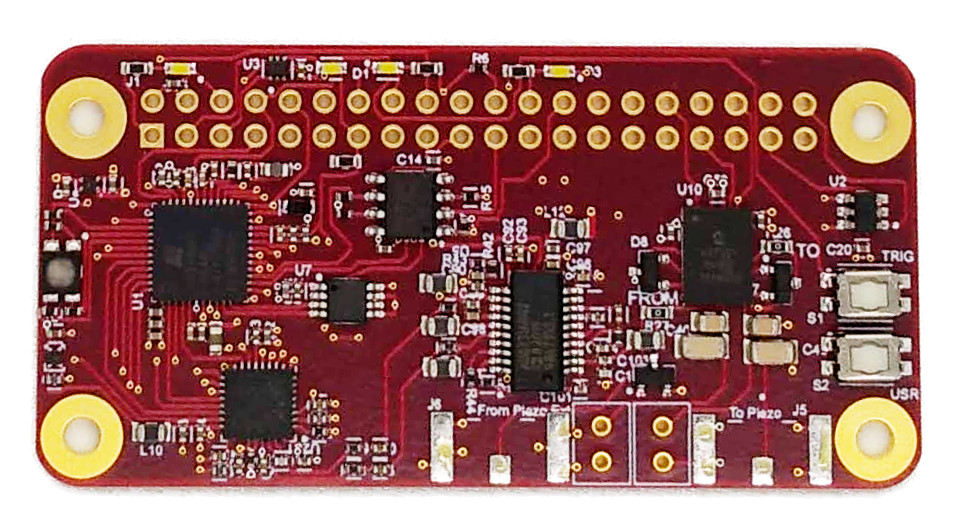
\includegraphics[width=.5\textwidth]{images/v1/top.jpg}\hfill
  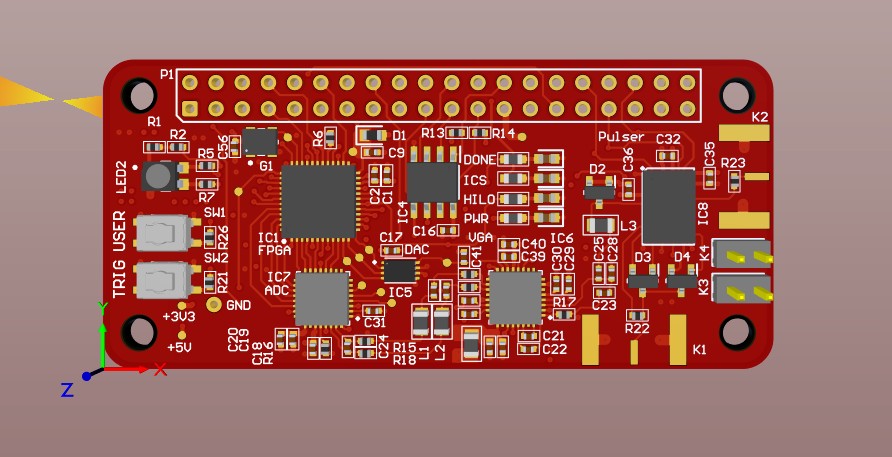
\includegraphics[width=.5\textwidth]{images/v2/top.png} 
  \caption{Top side of the lit3rick and its update, the lit3-32 boards.} 
  \label{fig:images}
  \end{figure}
 

\subsection{Concept}

\textbf{FPGA:} a Lattice up5K chip: chosen as the right compromise between a number of IOs, RAM, and fabric speed. It is compatible with Claire  Wolf's \href{http://www.clifford.at/yosys/}{Yosys} Open SYnthesis Suite. 

\textbf{Memory:}  FPGA RAM - 1Mb, as well as 8 Mb SPI Flash for FPGA configuration. It gets filled with a AD9629BCPZ-65, 64Msps ADC.

\textbf{Ultrasound processing: } A VGA (AD8331 for the lit3rick, AD8332 for the lit3-32) controled by DAC, with a HV7361GA pulser (bipolar, +- 100V). The VGA allows in the first case an amplification in the +7.5 dB to +55.5 dB range, while the second range of the AD8332 allows to reach 84.5dB.
        
\textbf{Extensibility:}  two SMA plug for the piezos (with capacity to separate the TX and RX paths) as well as a general header for RPi GPIO

\textbf{User Interfaces:} a RGB LED, 2 push button (with software noise debouncing) and jumpers for high voltage selection, connected to the TX/RX and I2C pins of the RPi header. The header i2s IOs are also connected, allowing for exporting signals through this audio bus.

\textbf{Input Voltage:} 5 V from RPi or USB, uses 350mA-450mA at 5V with a raspberry on. The FPGA and logic operate at at 3.3 V. For cost-efficiency, the high voltage generation component was removed from the board.

\section{Where to find the latest sources} 
 

The latest sources of the hardware as well as software are available at \url{https://github.com/kelu124/lit3rick/}. However, this PDF also doubles as an archive (you can rename the .pdf as a .zip, and you'll see), and contains, in short: a set of gerbers and BOM, some VHDL/verilog code, a basic FPGA binary ready to be used, and a python library to operate the board from a Raspberry Pi. There may be some other stuff there, but I forgot what I put there.

\section{Operation} 

The FPGA has all the right logic in place to provide you with a full control over the pulse-echo process. At the time of this paper, the verilog had been developed for the lit3rick, but not for the lit3-32 board.

\begin{figure}[htp!]
  \centering
  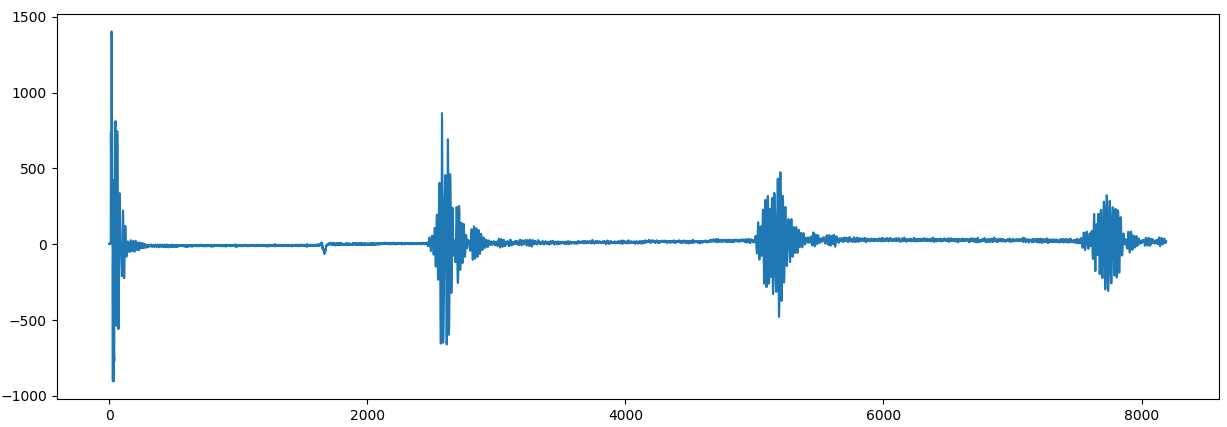
\includegraphics[width=.98\textwidth]{images/v1/raw_ref.png}\hfill 
  \caption{Example of raw signal acquisition on the lit3rick.} 
  \label{fig:lit3rick}
  \end{figure}

We have demonstrated the possibility as well to provide an onboard filtering, enveloppe detection and enveloppe compression, using an A-Law approach. 


\begin{figure}[htp!]
  \centering
  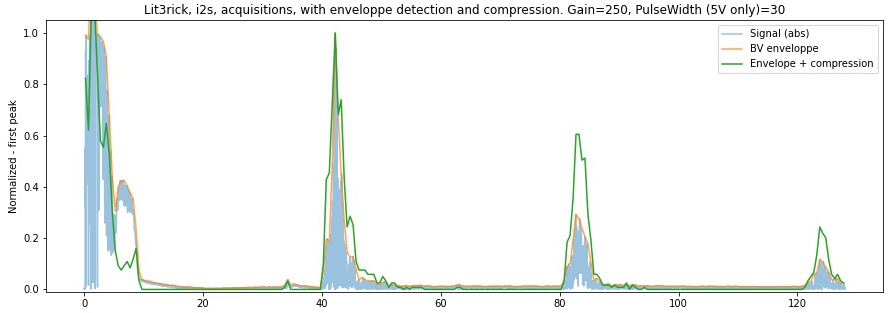
\includegraphics[width=.98\textwidth]{images/v1/lit3_i2s.jpg}\hfill 
  \caption{Example of enveloppe detection acquisition.} 
  \label{fig:i2s}
  \end{figure}


 
\newpage \section{Last details}
\paragraph{Certification}

The lit3rick and lit3-32 boards are also open-hardware certified, respectively under ID \href{https://certification.oshwa.org/fr000006.html}{FR000006} and ID \href{https://certification.oshwa.org/fr000016.html}{FR000016}.


\paragraph{License}

This work is based on previous TAPR projects, the un0rick and the echOmods projects. The lit3rick project and its boards are open hardware and software, developed with open-source elements.

Copyright kelu124 (kelu124@gmail.com) 2018

\begin{itemize}
\item The hardware is licensed under TAPR Open Hardware License (www.tapr.org/OHL)
\item The software components are free software: you can redistribute it and/or modify it under the terms of the GNU General Public License as published by the Free Software Foundation, either version 3 of the License, or (at your option) any later version.
\item The documentation is licensed under a Creative Commons Attribution-ShareAlike 3.0 Unported License.
\end{itemize}


\section{Links to go further}

\begin{itemize}
\item Come and chat : \href{https://join.slack.com/usdevkit/shared_invite/MTkxODU5MjU0NjI1LTE0OTY1ODgxMDEtMmYyZTliZDBlZA}{join the Slack channel} 
\item The \href{https://github.com/kelu124/lit3rick}{ full GitHub Repo} with more ongoing works : also \href{https://github.com/kelu124/echomods/}{a messy braindump with all experiments} 
\item The board’s \href{https://www.tindie.com/stores/kelu124/}{Tindie shop} to get it
\item The project \href{https://hackaday.io/project/28375-un0rick-an-ice40-ultrasound-board}{ Hackaday page} with more logs
\item Check out \href{https://openhardware.metajnl.com/articles/10.5334/joh.2/}{my previous work} on the topic of ultrasound modules \cite{kelu124} and its \href{http://doi.org/10.5281/zenodo.377054}{dataset on Zenodo}. More to come!

\end{itemize}

 \section{Next steps}

Plenty to do on the next steps! Let me know if you'd like to contribute. The current shopping list (non-exhaustive) may include:

\begin{itemize}
\item Improving the documentation, and updated the work of its \href{https://github.com/kelu124/un0rick}{predecessor, the un0rick} \cite{un0rick}.
\item Work on BOM costs and overall hardware design.
\item Increase the high voltage source, and have it settable via an on-board, and ideally have a bipolar design.  
\item Improving the features of the onboard firmware.. and try to develop a VGA output ! So far, we have put a small micropython design up and running.
\item Work on the FTDI - so I have only used the RPi, and write something to program the flash from the RPi. 
\end{itemize}


\bibliographystyle{unsrt}  
%\bibliography{references}  %%% Remove comment to use the external .bib file (using bibtex).
%%% and comment out the ``thebibliography'' section.


%%% Comment out this section when you \bibliography{references} is enabled.
\begin{thebibliography}{1}

  \bibitem{kelu124}
  Luc Jonveaux 2017.
  \newblock  Arduino-like development kit for single-element ultrasound imaging. 
  \newblock In {\em  Journal of Open Hardware, 1(1), p.3}. DOI: \href{http://doi.org/10.5334/joh.2}{10.5334/joh.2}
  
  \bibitem{pyusb}
  Luc Jonveaux 2018.
  \newblock The pyusbus repository.
  \newblock Website at {\em\href{https://github.com/kelu124/pyusbus}{https://github.com/kelu124/pyusbus}}
  
  \bibitem{un0rick}
  Luc Jonveaux 2019.
  \newblock  un0rick : open-source fpga board for single element ultrasound imaging
  \newblock On {\em  Zenodo}. DOI: \href{http://doi.org/10.5281/zenodo.3364559}{10.5281/zenodo.3364559}
  
  \bibitem{lit3rick}
  Luc Jonveaux 2021.
  \newblock lit3rick: an up5k ultrasound pulse-echo device %%@todo change title
  \newblock On {\em  Zenodo}. DOI: \href{http://doi.org/10.5281/zenodo.5792245}{10.5281/zenodo.5792245}
  
  \bibitem{mux}
  Luc Jonveaux 2021.
  \newblock An open-source max14866 development board %%@todo change title
  \newblock On {\em  Zenodo}. DOI: \href{http://doi.org/10.5281/zenodo.5792252}{10.5281/zenodo.5792252}
  
  \bibitem{probes}
  Luc Jonveaux 2021.
  \newblock  pyubus: opening usb ultrasound probes  %%@todo change title
  \newblock On {\em  Zenodo}. DOI: \href{http://doi.org/10.5281/zenodo.5792256}{10.5281/zenodo.5792256}
  
\end{thebibliography}

\end{document}


% Subertley     
%                                             
%  .__  .__  __ ________       .__        __    
%  |  | |__|/  |\_____  \______|__| ____ |  | __
%  |  | |  \   __\_(__  <_  __ \  |/ ___\|  |/ /
%  |  |_|  ||  | /       \  | \/  \  \___|    < 
%  |____/__||__|/______  /__|  |__|\___  >__|_ \
%                      \/              \/     \/
%  